\chapter{Arrays}

Consider this snippet of code:

\begin{code}
if      (day ==  0) System.out.println("Monday");
else if (day ==  1) System.out.println("Tuesday");
else if (day ==  2) System.out.println("Wednesday");
else if (day ==  3) System.out.println("Thursday");
else if (day ==  4) System.out.println("Friday");
else if (day ==  5) System.out.println("Saturday");
else if (day ==  6) System.out.println("Sunday");
\end{code}

\noindent What does this code do? It prints the day of the week after conditioning on the value of an integer \ic{day}. But this code is repetitive. It would be useful if we had some way of creating a list of days of the week, and then just specifying which of those days we wanted to print. Something like this:

\begin{code}
System.out.println(DAYS\_OF\_WEEK[day]);
\end{code}

To achieve this in Java, we need arrays.

\begin{definition}
An \emph{array} is an ordered and fixed-length list of values that are of the same type. We can access data in an array by \emph{indexing}, which means referring to specific values in the array by number. If an array has \ic{n} values, then we think of it as being numbered from \ic{0} to \ic{n-1}.
\end{definition}

\begin{figure}
	\centering
	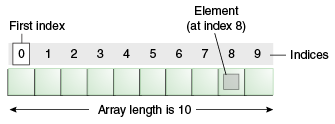
\includegraphics[width=0.5\textwidth]{images/array-diagram.png}
	\caption{Diagram of an array (Credit: https://www.geeksforgeeks.org/arrays-in-java/)}
\end{figure}

To \emph{loop} or \emph{iterate} over an array means that our program accesses every value in the array, typically in order. For example, if we looped over the array in the diagram, that would mean that we looked at the value at the 0th index, then the value at the 1st index, then the value at the 2nd index, and so on.

When we say that the array is "ordered" is that the relationship between an index and its stored value is unchanged (unless we explicitly modify it). If we loop over an unchanged array multiple times, we will always access the same values.

Arrays are \emph{fixed-length}, meaning that after we have created an array, we cannot change its length. We will see in the next chapter [TK: confirm] that \ic{ArrayLists} are an array-like data structure that allows for changing lengths.

Finally, all the values in an array must be of the same type. For example, an array can hold all floating point numbers or all characters or all strings. But an array cannot hold values of different types.

\section{Creating arrays}

The syntax for creating an array in Java has three parts:

\begin{enumerate}
\item Array type
\item Array name
\item Either: array size or specific values
\end{enumerate}

For example, this code creates an array of size \ic{n = 10} and fills it with all \ic{0.0}s

\begin{code}
double[] arr;                    // Declare array
arr = new double[n];             // Initialize the array
for (int i = 0; i < n; i++) {    // Iterate over array
    arr[i] = 0.0;                // Initialize elements to 0.0
}
\end{code}

The key steps are: we first declare and initialize the array. We then loop over the array to initialize specific values. We can also initialize the array at compile time, for example

\begin{code}
String[] DAYS_OF_WEEK = {
//  Indices:
//  0      1      2      3      4      5      6
    "Mon", "Tue", "Wed", "Thu", "Fri", "Sat", "Sun"
};
\end{code}

Notice the difference in syntax. When creating an empty array, we must specify a size. When initialize an array at compile time with specific values, the size is implicit in the number of values provided.

Finally, in Java, it is acceptable to move the brackets to directly after the type declaration to directly after the name declaration. For example, these two declarations are equivalent:

\begin{code}
int arr[];
int[] arr;
\end{code}

\section{Indexing}

Consider the array \ic{DAYS\_OF\_WEEK} from the previous section. We can \emph{index} the array using the following syntax:

\begin{code}
System.out.println(DAYS_OF_WEEK[3]);  // Prints "Thu"
\end{code}

In Java, array's are said to use \emph{zero-based indexing} because the first element in the array is accessed with the number \ic{0} rather than \ic{1}.

\begin{example}
What does \ic{System.out.println(DAYS\_OF\_WEEK[1]);} print?
\end{example}

\begin{example}
What does this code do? What number does it print?

\begin{code}
double sum = 0.0;
double[] arr = { 1, 2, 2, 3, 4, 7, 9 }
for (int i = 0; i < arr.length; i++) {
    sum += arr[i];
}
System.out.println(sum / arr.length);
\end{code}
\end{example}

\section{Array length}

As mentioned previously, arrays are \emph{fixed-length}. After you have created an array, it's length is unchangeable. You can access the length of an array \ic{arr[]} with the code \ic{arr.length}.

\begin{example}
What does \ic{System.out.println(DAYS\_OF\_WEEK.length);} print?
\end{example}

\begin{example}
Write a \ic{for} loop to print the days of the week in order (Monday through Sunday) using an array rather than seven \ic{System.out.println} function calls.
\end{example}

\section{Default initialization}

In Java, the default initial values for numeric primitive types is \ic{0} and \ic{false} for the \ic{boolean} type.

\begin{example}
Consider this code from earlier:

\begin{code}
double[] arr;
arr = new double[n];
for (int i = 0; i < n; i++) {
    arr[i] = 0.0;
}
\end{code}

Rewrite this code to be a single line.
\end{example}

\section{Bounds checking}

Consider this snippet of code.

\begin{example}Where is the bug?
\begin{code}
int[] arr = new int[100]; 
for (int i = 0; i <= 100; ++i) {
    System.out.println(arr[i]);
}
\end{code}
\end{example}

The issue is that the program attempts to access the value \ic{arr[100]}, while the last element in the array is \ic{arr[99]}.

This kind of bug is called an ``off-by-one error'' and is so common it has a name. In general, an off-by-one-error is one in which a loop iterates one time too many or too few.

\begin{example}
Where is the off-by-one-error?

\begin{code}
int[] arr = new int[100];
for (int i = 0; i < array.length; i++) {
    arr[i] = i;
}
for (int i = 100; i > 0; --i) {
    System.out.println(arr[i]);
}
\end{code}
\end{example}

\begin{example}
Fill in the missing code in this \ic{for} loop to print the numbers in reverse order, i.e. \ic{5, 4, 3, 2, 1}:

\begin{code}
int[] arr = { 1, 2, 3, 4, 5 };
for (???) {
    System.out.println(arr[i]);
}
\end{code}
\end{example}

\section{Empty arrays}

This code prints five values, one per line, but we never specified which values. What do you think it prints?

\begin{code}
int[] arr = new int[5];
for (int i = 0; i < arr.length; i++) {
    System.out.println(arr[i]);
}
\end{code}

In Java, an unitialized or empty array is given a default value:

\begin{itemize}
\item For \ic{int}, \ic{short}, \ic{byte}, or \ic{long}, the default value is \ic{0}.
\item For \ic{float} or \ic{double}, the default value is \ic{0.0}
\item For \ic{boolean} values, the default value is \ic{false}.
\item For \ic{char}, the default value is the null character \ic{'\u0000'}.
\end{itemize}

Note that an array can be partially initialized.

\begin{example}
What does this code print?

\begin{code}
char[] alphabet = new char[26];
alphabet[0] = 'a';
alphabet[1] = 'b';
for (int i = 0; i < alphabet.length; i++) {
    System.out.println(alphabet[i]);
}
\end{code}
\end{example}

\section{Enhanced for loop}

So far, we have seen how to iterate over arrays by indexing each element with a number:

\begin{code}
char[] vowels = {'a', 'e', 'i', 'o', 'u'};
for (int i = 0; i < vowels.length; ++ i) {
    System.out.println(vowels[i]);
}
\end{code}

We can perform the same iteration without using indices using an ``enhanced \ic{for} loop'' or \ic{for-each} loops:

\begin{code}
char[] vowels = {'a', 'e', 'i', 'o', 'u'};
for (char item: vowels) {
    System.out.println(item);
}
\end{code}

\section{Exchanging and shuffling}

Two common tasks when manipulating arrays are \emph{exchanging two values} and \emph{shuffling} values. (\emph{Sorting} is more complicated and will be address later.)

To exchange to values, consider the following code:

\begin{code}
double[] arr = { 1.0, 2.0, 3.0, 4.0, 5.0, 6.0 };
int i = 1;
int j = 4;
double tmp = arr[i]; 
arr[i] = arr[j]; 
arr[j] = tmp;
\end{code}

\begin{example}
What are the six values in the array, in order?
\end{example}

To shuffle the array, consider the following code:

\begin{code}
int n = arr.length; 
for (int i = 0; i < n; i++) { 
    int r = i + (int) (Math.random() * (n-i)); 
    String tmp = arr[r];
    arr[r] = arr[i];
    arr[i] = tmp;
}
\end{code}

\begin{example}
What does this code do:

\begin{code}
for (int i = 0; i < n/2; i++) {
    double tmp = arr[i];
    arr[i] = arr[n-1-i];
    arr[n-i-1] = tmp;
}
\end{code}
\end{example}

\exercisesection

\begin{exercise}
Write a program that reverses the order of values in an array.
\end{exercise}

\begin{exercise}
What is wrong with this code snippet?

\begin{code}
int[] arr;
for (int i = 0; i < 10; i++) {
    arr[i] = i;
}
\end{code}
\end{exercise}

\begin{exercise}
Rewrite this snippet using an enhanced \ic{for-each} loop (for now, it is okay to re-define the array):

\begin{code}
char[] vowels = {'a', 'e', 'i', 'o', 'u'};
for (int i = array.length; i >= 0; i--) {
    char letter = vowels[i];
    System.out.println(letter);
}
\end{code}
\end{exercise}

\begin{exercise}
Write a program that uses \ic{for} loops to print the following pattern:

\begin{code}
1********

12*******

123******

1234*****

12345****

123456***

1234567**

12345678*

123456789
\end{code}
\end{exercise}

\begin{exercise}
Write a program \ic{HowMany.java} that takes an arbitrary number of command line arguments and prints how many there are.
\end{exercise}

\referencessection

Computer Science: An Interdisciplinary Approach, Robert Sedgewick and Kevin Wayne.
